\newpage
\section{Alarm og feilhandtering}
\thispagestyle{fancy}

% Skriver litt om introduksjon om alarm og feilhandtering
Alarm og feilhandtering utgjer ein sentral del av eit velfungerande styresystem. Det er avgjerande
at anlegget effektivt handterer og varslar om uønskte hendingar, slik at 
driftspersonalet blir varsla og nødvendige tiltak kan raskt setjast i verk.

% Skrive litt om codesys alarmhantering
For å varsle om alarm og feil i vårt program, har vi nytta oss av \gls{Codesys} sine
innebygde alarmhandteringsfunksjonar \citep{CodesysAlarm}. Desse funksjonane gir oss høve til å 
kontrollere, gruppere og prioritere alarmar, samt å sende informative tekstar til driftspersonalet.

% Skriver om alarmar både gamle og nye.
\gls{IEC}-blokkene som vi har utvikla, gir oss moglegheita til å detektere ulike typar hendingar
som feil, alarmar og forvarsel.
Dei forskjellige blokkene har ein variert mengde med feil som skal kunne detekterast og varslast.
Forløpet er slik at feil blir detektert og ein boolsk variabel \gls{YF} blir sett til ``true'', 
samt at ein heiltalsverdi \gls{YFI} indikera kva type feil som har inntruffe.\newline
Alle desse moglege typane varslingar, som er omtala i vedlegg E, 
er samla i programmet vårt saman 
med dei aktive varslingane som er i bruk på Sande reinseanlegg i dag.

Vi har valt å dele opp alle varslingane i fire forskjellige grupper:

\begin{itemize}
    \item \textbf{Feil}          (Der systemet ikkje fungera, t.d. sensorfeil og blokkfeil)
    \item \textbf{Alarmar}       (Kritiske prosessparametrar, t.d. straumbrot og veldig høge nivå)
    \item \textbf{Forvarsel}     (prosessparametrar som nærmar seg kritisk nivå)
    \item \textbf{Informasjon}   (Prosessinformasjon med nytteverdi)
\end{itemize}

Ved å kategorisere varslingar i fire ulike grupper med forskjellige prioriteringsnivå,
vil systemet og driftspersonalet enklare kunne forstå samanhengen og alvoret i varslingane. \newline
Korleis dei ulike alarmane blir definert og prioriterte må evaluerast i samråd med \gls{Sunnfjord Kommune}.




\begin{figure}[htbp]
    \centering
    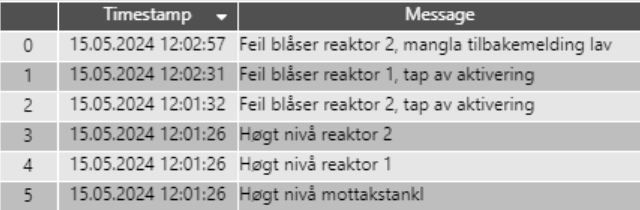
\includegraphics[width=0.6\textwidth]{Bilder/Alarmeksempel.png}
    \caption{Alarmlogg implimentert i programmet}\label{fig:Alarmlogg}
\end{figure}

\newpage

